\chapter{Analyse des opportunités des technologies libres dans le
domaine de l'édition vidéo et prévisions}

\minitoc \newpage

\paragraph{}

Maintenant que les besoins et que les solutions existantes ont été
analysées on rendra compte de la situation actuelle des technologies
libres et de leurs communautés. Il est aussi important de chercher
les raisons qui expliquent que ces logiciels ne sont pas plus utilisés
par les professionnels. Puis, nous essayerons d'envisager les solutions
possibles qui permettraient de remédier à cette situation.

\paragraph{}

Dans cette partie, nous analyserons la différence entre les manières
d'envisager la création de logiciel et nous verrons quels sont les
avantages et inconvénients de ces fonctionnements. Par la suite nous
nous concentrerons sur les frameworks existants pour faire une analyse
technique de ces technologies. Puis, nous analyserons les communautés
qui portent ces différents projets afin de déterminer les points forts
et les points faibles de chacun des projets.  Pour finir, nous tirerons les
conclusions de cette analyse afin de trouver des solutions aux défis
qu'est la création d'un logiciel libre de montage vidéo.

\newpage

\section {Etat actuel de l'offre de logiciel libre}

Le schéma suivant permet de résumer facilement la situation:

\begin{figure} [h]
  \begin{center}
    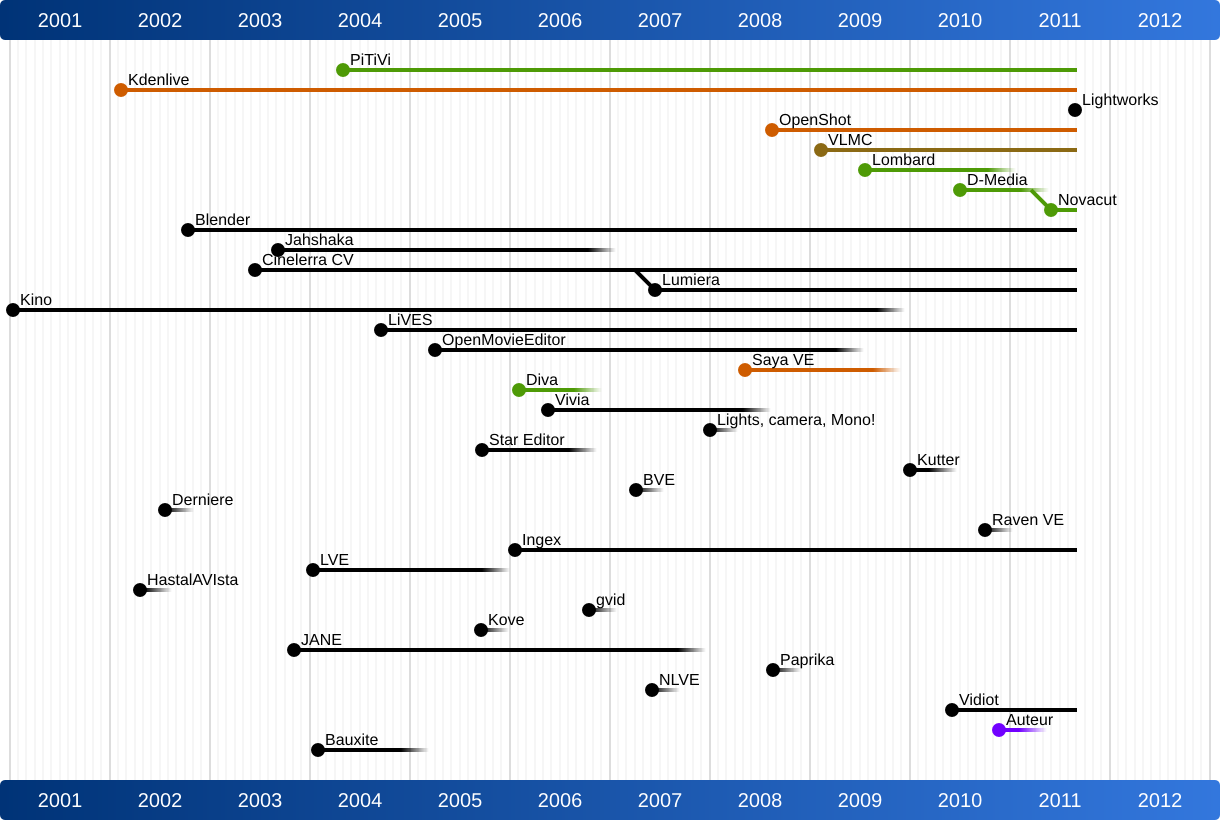
\includegraphics[width=0.9\textwidth]{images/open-source-video-editor-timeline}
  \end{center} \caption{Open source video editors timeline (Auteur:
  Jean-François Fortin, PiTiVi designer)} \label{Yes}
\end{figure}

\paragraph{ }

On constate donc que de nombreux projets de logiciel libre de montage
vidéo on vu le jours ces 10 dernières années% et dont les objectifs sont différents
.  On peut distinguer deux types de public visés par ces projets:

\begin {itemize}

  \item {Les amateurs}

  \item {Les professionnels ou semi professionnels}
\end {itemize}

\paragraph {Les amateurs de montages vidéo}

\subparagraph{}

Plusieurs projets libres permettent ou visent à répondre aux besoins
des amateurs, mais à l'heure actuelle %ils ne sont que partiellment adaptés à ces besoins.
. Parmi les logiciels dont l'objectif est de permettre de créer des montages
simples on distingue:

\begin {itemize}

  \item {openshot: Logiciel présentant  de nombreuses fonctionnalités,
  mais dont la
    qualité d'implémentation présente des faiblesses.}

  \item {kino: Logiciel avec un nombre de fonctionnalités limité
  permettant de faire des
    petit montages %avec efficacité.}

  \item {Vidiot qui vise la production de vidéo amateur simple}

\end {itemize}

\paragraph {}

Mais %il existe des logiciels ayant pour objectif de %répondre aux besoins plus
avancés en particulier à ceux des professionnels (précédemment
présenté dans le cadre de la définition des plus grands acteurs du
marché) % qui peuvent être utilisés dans le cadre de montage amateur. 
%Leur utilisation (et c'est plus particulièrement le cas du logiciel Cinelerra)
%demeure complexe.

\paragraph{}

Un nouveau projet a aussi récemment vu le jour, dont la finalité est
assez différente des logiciels actuellement présents. Il s'agit de
Novacut, qui permet aux créateurs de films et séries web de faire le
montage de manière collaborative %avec Internet en partageant
les ressources (footage).

\paragraph{}

% Human readable version:

% Le fait que Cinelerra ne soit packagé dans aucune distribution

% Linux montre que même ce logiciel est le seul à avoir réussi à

% prendre une part de marché dans le milieu de l'édition

% professionnelle, celui-ci n'a pas réussi à rassembler les

% développeurs et utilisateurs standard de logiciel libre.

Le fait que Cinelerra ne soit packagé \footnote{Packagé: fait
que qu'un paquet, une archive (fichier compressé) comprenant les
fichiers informatiques, les informations et procédures nécessaires
à l'installation d'un logiciel sur un système d'exploitation au sein
d'un agrégat logiciel, en s'assurant de la cohérence fonctionnelle
du système ainsi modifié ait été créé. Source: Wikipedia} dans
aucune distribution Linux \footnote {Une distribution Linux, appelée
aussi distribution GNU/Linux pour faire référence aux logiciels du
projet GNU, est un ensemble cohérent de logiciels, la plupart étant
logiciels libres, assemblés autour du noyau Linux. Source: Wikipedia}
montre que même ce logiciel est le seul à avoir réussi à prendre une
part de marché dans le milieu de l'édition professionnel, celui-ci n'a
pas réussi à rassembler les développeurs et utilisateurs standard de
logiciel libre.

\paragraph{}

En définitive aucun projet n'a encore réussi à s'imposer et ainsi
regrouper les développeurs au sein de projets majeurs. Dans d'autre
domaines, cela a été le cas, par exemple dans le domaine des lecteurs
vidéo, Vlc a su surpasser ses concurrents, et ainsi supplanter le
marché des lecteurs vidéo, qu'il soit libre ou non. Dans le domaine
des environnements de Bureau graphique, KDE et Gnome sont arrivés à un
stade où leur supériorité technique, et en terme de fonctionnalités,
fait d'eux des plateformes de référence.

\paragraph{}

Il est donc intéressant de se demander quelles technologies et quels
logiciel(s), pourraient se voir attribuer cette place dans le monde
de l'édition vidéo libre. Nous allons donc analyser les logiciels et
les technologies libres les plus avancés, (précédemment mentionnés
dans le cadre de l'analyse de marché: Cinelerra, Kdenlive et PiTiVi).
Nous verrons ainsi s'ils ont le potentiel de pouvoir un jour rivaliser
avec les logiciels propriétaires sur le marché très fermé du montage
vidéo professionnel.

\paragraph{}

NB: Il aurait été intéressant d'analyser le logiciel lightworks,
en voie de libération, mais à l'heure actuelle, aucun code n'a été
libéré, et par conséquent, celui-ci ne peut pas faire partie de
cette analyse.

\newpage

\section{Technologies}

\paragraph{}

Pour faire une analyse technique des produits permettant de faire
de l'édition vidéo, il est nécessaire d'analyser le ``core'' des
logiciels, c'est à dire la partie du logiciel où les opérations
d'édition sont effectivement réalisées. Dans ces domaines, il existe
deux façon de procéder:

\begin{itemize} \setlength{\itemsep}{2mm}

  \item{Création d'un logiciel monolithique\index{monolithique}}

  \item{Création d'un framework \glossary {name={framework},
   description={Un framework est un ensemble d'outils et de composants
   logiciels organisés conformément à un plan d'architecture et des
   designs patterns (un patron de conception, motif de conception ou
   modèle de conception est un concept de génie logiciel destiné à
   résoudre les problèmes récurrents suivant le paradigme objet.)}}
   \index{framework}}

\end{itemize}

\subsection {Technologies monolithiques\index{monolithique} VS
technologies modulaires, frameworks}


\subsubsection{Logiciels monolithiques \index{monolithique}}

\paragraph{}

Le conception monolithique \index{monolithique} dans le cadre des
logiciels d'édition vidéo, consiste à développer au sein d'un même
entité de code:

\begin{itemize} \setlength{\itemsep}{2mm}

  \item {la partie graphique et la partie de calculs
    permettant la gestion de tout ce que l'édition non linéaire
    implique}

  \item {L'interface utilisateur.}

\end {itemize}

\paragraph{}

Par le terme logiciel monolithique\index{monolithique}, il faut réaliser
que le logiciel peut utiliser des librairies externes, mais le core de
ce même logiciel, et la logique d'édition linéaire à proprement
parler sont directement %élaborés à l'intérieur du logiciel et non par
une librairie ou framework \index{framework} externe. Cela a pour
principal avantage de présenter une conception simplifiée pour les
raisons suivantes:

\paragraph{}

Les logiciels professionnels (commerciaux) utilisent très probablement
tous ce mode de fonctionnement (même si vraisemblablement, en interne il ont
un core qui ressemble fortement à un framework \index{framework}).Dans
le monde des logiciels libres,les développeurs de Cinelerra ont décidé
d'utiliser ce mode de fonctionnement.

On peut voir plusieurs conséquences immédiates de ce mode de
développement:

\begin{itemize} \setlength{\itemsep}{2mm}

  \item {Les développeurs n'ont pas la nécessité de penser
    en terme d'interface publique de programmation (API\index{API}), et
    n'ont pas à garantir la stabilité de celle-ci: le risque réside
    dans le fait que la qualité de l'architecture ne soit pas optimale
    car la création d'API\index{API} oblige les développeurs/architectes
    à réellement analyser les besoins de manière plus large dès
    le début de la conception. Dans le cas où l'on ne crée pas
    d'interface publique de programmation vouée à être réutilisée,
    le risque est que le travail de design et d'architecture ne soit
    pas réalisé, et que le code grandisse de manière anarchique avec
    les différents développeurs qui font des extensions au fur et à
    mesure de leurs besoins.}

  \item {Les développeurs n'ont besoin de penser l'architecture seulement
  pour les cas d'utilisation qui sont liés à ce même logiciel:
    ils n'ont pas à voir au delà de ces use cases.}

  \item {Les erreurs en terme de design n'ont pas d'incidences aussi
    graves que dans le cas d'un framework\index{framework}.}
\end {itemize}

\paragraph{}

On se rend compte que cette manière de faire a pour principal avantage
le fait que le logiciel peut être développé plus rapidement puisque
le core du logiciel, et donc le code qui implémente la logique de
l'édition non linéaire, est conçue avec pour seul cas d'utilisation,
celui du logiciel. Cependant, de nombreux inconvénients existent à
cause de la nature monolithique\index{monolithique} du design:

\subparagraph{Besoins en main d'oeuvre considérables:}

\subparagraph { }

Dans le cadre de logiciel d'édition vidéo, le code à produire est
considérable, comme le montre les statistiques (Annexes 2). Le logiciel
Cinelerra à lui seul fait plus d'un million de lignes. Une telle
quantité %(je dirai plutôt "un tel volume")de code est difficile à maintenir et requiert des ressources
importantes en terme de main d'oeuvre. Le fait que le logiciel soit
monolithique\index{monolithique} implique que celui-ci va être utilisé
seulement par ce logiciel, et par conséquent, les développeurs ne
peuvent pas compter sur d'autre utilisation de ce code pour améliorer
et développer le core du logiciel.

\paragraph{Réutilisabilité:}

\subparagraph { }

L'un des inconvénients de cette manière de faire est que le code %présent
 à l'intérieur du logiciel n'est pas réutilisable directement
par d'autres projets. %On le considère comme
``individualiste``, %situation qu'il convient d'éviter dans le cadre du
développement de logiciel libre afin de ne pas multiplier les efforts,
et dupliquer le code.

\paragraph{}

Cette façon de faire a été utilisée par le projet Cinelerra. Ce
logiciel est le plus avancé en terme de fonctionnalités %dans l'offre 
des logiciels libres de montage . On peut penser que son
architecture monolithique\index{monolithique} explique ce développement
plus abouti, bien qu'il y ait évidemment de nombreux autres facteurs qui
interviennent, en particulier le fait que ce logiciel ait été développé
par la société Heroine Virtual.

\subsubsection {Utilisation de  frameworks \index{framework}}

\paragraph{}

L'autre possibilité est de séparer en deux parties bien distinctes
l'implémentation de la logique de l'édition, lecture, encoding vidéo
(core logiciel), de la partie graphique, interaction avec l'utilisateur
final.

\paragraph {Le framework}

\subparagraph{}

La grande différence entre la conception monolithiques
\index{monolithique} et la création d'un framework \index{framework}
réside dans le le fait que dans le cadre d'un framework, on développe
une API \index{API} autour du core du logiciel. Cela résulte dans le
fait que le core est un programme (librairie) externe, réutilisable par
n'importe quel autre application.  On peut considérer que les avantages
des frameworks sont les inconvénients des applications monolithiques
\index{monolithique} et vice-versa. L'avantage principal des frameworks
sur une conception monolithique\index{monolithique} est la possibilité
de partager un même code à travers de multiples applications. Celà
permet de réunir les efforts au travers, dans notre cas précis, de
tout type d'application multimedia.

\subparagraph{}

Dans le cadre de l'édition vidéo, on peut encore distinguer deux
manière d'envisager son développement:

\begin {itemize}

  \item {Utiliser un framework multimedia généraliste, et créer les
  outils nécessaire
         au montage au dessus de celui-ci} %stupid french!\ldots On top
                                           %of it?

  \item {Créer un framework spécialement orienté montage vidéo}

\end {itemize}

\subparagraph{}

Dans le monde du logiciel libre, ces deux manières d'envisager le
développement d'un framework multimedia ont été abordées par les
deux projets de framework leader sur ce segment:

\begin {itemize}

  \item {MLT qui se définit comme étant un ``Framework multimedia design
    et développé pour le broadcasting télévisé.''}

  \item {Gstreamer qui se définit comme étant un ``framework multimédia
    basé sur la notion de pipeline" ce qui lui permet de nombreux types
    d'applications multimedia tels que des lecteurs multimédia, des
    logiciels de broadcasting, des logiciels de montage vidéo\ldots''}

\end {itemize}

\subparagraph {}

Au dessus de ces frameworks, plusieurs applications (interfaces graphiques)
de montage vidéo se sont développées.

\begin {itemize}

  \item {PiTiVi: utilise le Framework multimedia GStreamer}

  \item {Kdenlive openshot utilisent le framework\index{framework}
  orienté édition et broadcasting MLT.}

\end {itemize}

\paragraph {}

Dans le cadre des Frameworks, nous nous intéresserons en particulier
à l'analyse de ceux-ci puisque les notions relatives à l'édition
vidéo, et la gestion de toute la partie multimédia est réalisée
par ceux-ci. Les logiciels d'édition ne sont à priori que de simples
interfaces graphiques basées sur ces frameworks. Dans les faits,
l'implémentation actuelle de PiTiVi n'est pas qu'un simple interface
graphique au dessus de GStreamer, mais une partie de la
logique d'édition vidéo est actuellement réalisée dans le logiciel même.
(ceci est en train de changer avec la migration \cite{PitviPortToGes}
vers gstreamer-editing-services\cite{PresentationOfGes}).

\newpage \section{Analyse technique}

\paragraph {}

Dans cette partie nous allons analyser les entrailles %(EST-CE UN TERME TECHNIQUE,, JE REMPLACERAI CE MOT "ENTRAILLES" PLUTÔT PAR "STRUCTURE" 
des trois logiciels
précédemment définis: Cinelerra, PiTiVi et Kdenlive.

\subsection{Cinelerra:}

Cinelerra est développé en C++ et utilise par conséquent la paradigm
objet.  Il est distribué sous licence GPL Version 2 ou plus.

\subsubsection{Documentation du code}

\subparagraph{}

Au niveau de la documentation, celle-ci est inexistante et le code
lui-même ne contient que très peu de commentaires. Il est donc très
compliqué de comprendre le fonctionnement et les relations entre ces
centaines de milliers de lignes de code. L'analyse de son fonctionnement
est par conséquent assez complexe, et il est possible que cette analyse
contienne des imperfections.

\subsubsection {Structuration du code}

En terme de structure, le code de Cinelerra est décomposé en 3 partie:

\begin{itemize}

  \item{Lecture, rendering  audio vidéo: ce code est principalement
    contenu dans les dossiers ``quicktime'', ``thirdparty'' et
    ``libmpeg3''.}

  \item{Effets audios et vidéos: Ceux-ci sont développés comme plugins,
    et le code est donc présent de le dossier ``plugins`` }

  \item{Edition vidéo non linéaire et interface graphique: ce code est
    contenu dans un seul et unique dossier, ``cinelerra''}

  \item{Système de plugins: Aussi développé dans le dossier
  ``cinelerra``}

\end{itemize}

\paragraph{}

Cette structure semble être assez limité puisqu'il convient en théorie
de décomposer le code par petites parties, alors que dans le cadre de
Cinelerra, le dossier ``cinelerra'' contient non  moins de 1000 fichiers
et 207789 lignes de code.

\subsubsection{Lecture, rendering}

\paragraph{}

Dans le cadre de la lecture audio et video, Cinelerra fait appel à
diverses librairies:

\begin{itemize}

  \item{ffmpeg: Solution compete, cross plateforme
  d'enregistrement, lecture, conversion de flux audio et vidéo. Il
  inclue libavcodec, librairie leader dans le domaines des
  coder/decoder\glossary{name={codec}, description={Un codec est un
  procédé
capable de compresser et/ou de décompresser un signal numérique. Ce
procédé peut être un circuit imprimé ou un logiciel.}}\index{codec}.
Il s'agit du core de la
  lecture audio et vidéo de Cinelerra.}

  \item{faac/faad: AAC audio encoder/decoder}

  \item{x264: h264 encoder}

  \item{libdv: DV codec}

  \item{\ldots}

\end{itemize}

\subparagraph{}

Toutes ces librairies sont utilisées dans le but de lire et écrire des
fichiers multimedia. Afin de standardiser, et permettre l'utilisation de
ces libraries de manière similaire au sein du logiciel, les développeurs
de Cinelerra ont élaboré au cas par cas des ponts entre ces librairies
et le reste du logiciel (Fichier dans le dossier quicktime).

\subparagraph{}

% humaine readable

%De plus, les créateurs de Cinelerra ont développé des librairies de

%codec\index{codec}, muxer et demuxer (En

%particulier Mpeg et quicktime) afin d'ameliorer l'utilisation de ces

%formats dans le cadre de l'édition vidéo. Cela a tout de même été

%effectué dans de librairies externes réutilisables par d'autres projets:

\begin{itemize}

% Human readable:

% Quicktime 4 Linux: supporte en particulier les formats DV,

% les codecs H.264 et AAC, et implémente des éléments de conversion

% d'espaces colorimétriques (colorspace conversion)

  \item {Quicktime 4 Linux: supporte en particulier les formats DV,
    les codecs H.264 et AAC, et implémente des éléments de conversion
    d'espaces colorimétriques (colorspace conversion)}

% Human readable

% Libmepg3: supporte la plupart des formats du ``Mpeg Picture

% Motion Group''  et permet l'édition vidéo en utilisant ces

% formats bien qu'il ne soit pas conçu pour ce type d'utilisation.

  \item {Libmepg3: supporte la plupart des formats du ``Mpeg Picture
    Motion Group'' \glossary{name={mpeg}, description={MPEG, sigle de
    Moving Picture Experts Group, est le groupe de travail SC 29/G 11
    du comité technique mixte JTC 1 de l’ISO et de la CEI pour les
    technologies de l’information. Ce groupe d’experts est chargé
    du développement de normes internationales pour la compression, la
    décompression, le traitement et le codage de la vidéo, de l’audio
    et de leur combinaison, de façon à satisfaire une large gamme
    d’applications. Source: Wikipedia}} et permet l'édition vidéo en
    utilisant ces formats bien qu'il ne soit pas conçu pour ce %type d'utilisation.}

\end{itemize}

\subsubsection {Effets audio et vidéo}

Afin de permettre la création d'effets, Cinelerra utilise du  code
provenant de deux librairies:

\begin{itemize}

  \item {ladspa, Linux Audio Developers Simple Plugins API: Librairie
  d'effets audios qui contient une multitude de plugins.Il s'agit d'une
  API très simple et extrêmement flexible qui théoriquement permet
  la création de plugins permettant n'importe quelle manipulation
  et transformation du son. Dans les faits, certaines
  fonctionnalités ne sont pas implémentées pour éviter de complexifier
  le core de la librairies.}

  \item {frei0r: Framework minimalist multi-platform de création
    d'effets vidéo. Il permet la création d'effets à travers des
    plugins. Il s'agit du standard de fait en terme d'effets vidéo
    dans le milieu des logiciels libres. Cette librairie a été
    %élaborée par de nombreux développeurs issus de différentes
    communautés de logiciels libres en relation avec le multimedia. De
    nombreux plugins existent et sont stables, mais %ils présentent un inconvénient
    assez important existe concernant ce set d'effet %car ils
    supportent uniquement l'espace de couleur RGB. Cela a pour
    conséquence que dans le cas ou le flux vidéo n'est pas dans
    cette espace de couleur,%CE N'EST PAS CLAIR COMME EXPLICATION\glossary {name={espace colorimétrique}
    description={Un espace colorimétrique ou espace de couleur associe
    des nombres aux couleurs visibles.  Compte tenu des limites de
    la vision humaine, ces nombres se présentent généralement sous
    la forme de triplets. Chaque couleur de lumière peut donc être
    caractérisée par un point dans un espace à trois dimensions. Lors
    d'une impression, pour des raisons liées à la qualité des
    pigments, l'espace utilisé comporte alors généralement au moins
    quatre dimensions. Source: Wikipedia}} une conversion d'espace
    colorimétrique est nécessaire afin de les utiliser. Un autre
    inconvénient de cette librairie %réside dans le fait que les effets sont réalisés de
    manière logicielle, alors qu'à l'heure actuelle, l'utilisation de la
    carte graphique permettrait de tirer partie de manière beaucoup
    plus intéressante dans l'application d'effets sur
    les vidéos.}

%SAMEDI SOIR


\end{itemize}

\paragraph{}

Afin de permettre l'utilisation d'effets, les développeurs de Cinelerra
on mis en place un système de plugins. En terme d'implémentation,
Cinelerra reprend le code de ces librairies dans un set de plugins
Cinelerra en ajoutant l'implémentation de l'interface graphique qui
permet la configuration de ces effets.

\subsubsection{Interface Graphique}

\paragraph{}

L'interface graphique est développée en utilisant directement le server
X sans aucune librairie graphique au dessus. Ceci a pour conséquence
d augmenter le code à produire mais permet de controller intégralement
le projet sans dépendre de ces librairies.  Dans le cadre de Cinelerra,
cela est %logique car ce logiciel est développé quasi intégralement
en interne.

\begin{figure} [H]

  \begin{center}

    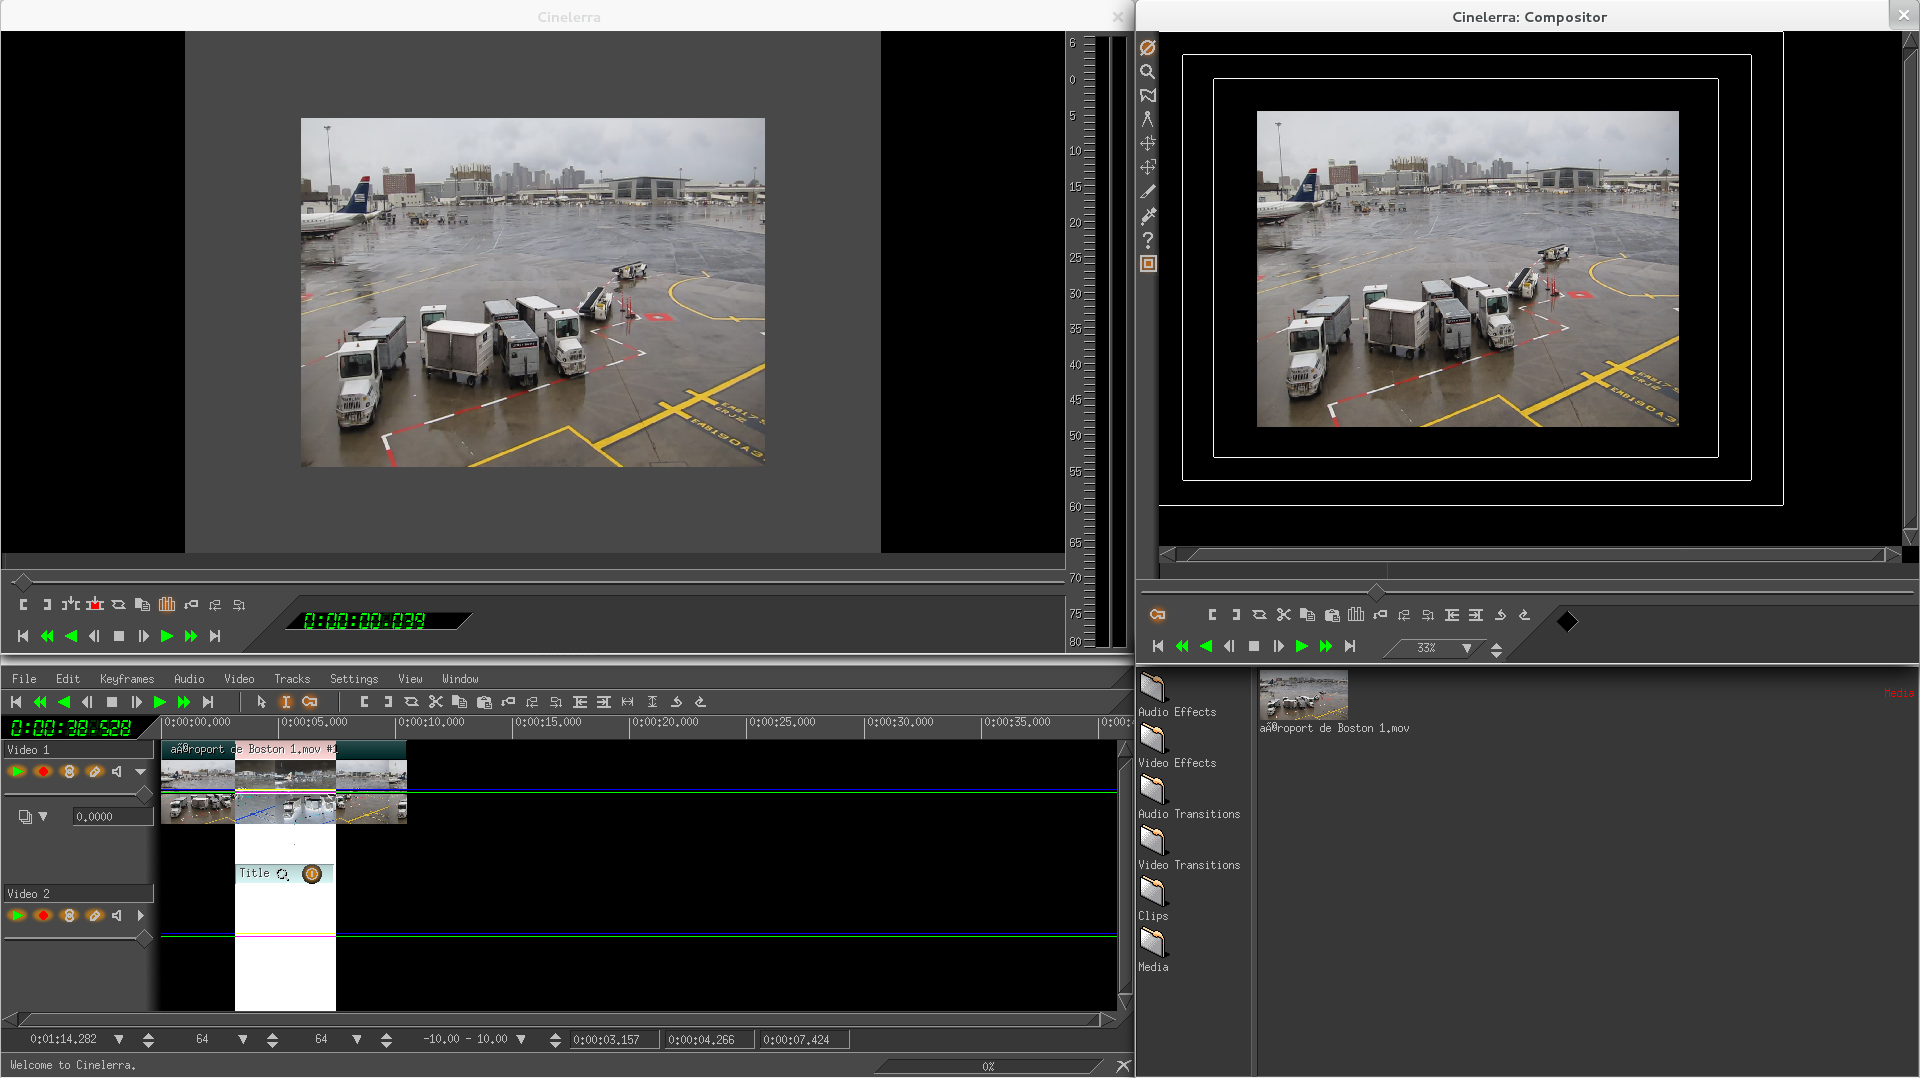
\includegraphics[width=0.95\textwidth]{images/cinelerra}

  \end{center}

  \caption{Interface graphique de cinelerra}

  \label{Yes}

\end{figure}

\paragraph{Structure de l'interface graphique:}

L'interface graphique de cinelerra est composée de quatre fenêtres
principales:

\begin{itemize}
  \item {La timeline (en bas à gauche sur le screenshot): cette
    partie permet de gérer un grand nombre d'%opérations sur le contenu de
    la timeline.}

  \item {La fenêtre de ressource (en bas à droite sur le screenshot):
    dans cette fenêtre l'utilisateur peut accéder au différents
    footages qu'il a importé. Il peut aussi accéder au différent effets,
    transitions\ldots}

  \item {Le fenêtre de preview (en haut à gauches sur le screenshot):
    cette fenêtre permet la prévisualisation des footages avant de les
    importer dans la timeline}

  \item {La fenêtre de composition (en haut à droite sur le screenshot):
    cette fenêtre permet d'effectuer des opérations sur les vidéos et
    de prévisualiser la timeline.}

\end{itemize}

\subsubsection{Edition non linéaire}

\paragraph{Conception}

\subparagraph{}

Dans Cinelerra, l'interface utilisateur et la logique de l'édition
vidéo sont deux parties %intégralement interdépendante. Au sein du
code, il n'est pas possible de savoir quelle partie est plutôt liée à
l'interface graphique et quelle partie %réalise les calculs. Ceci est dû 
%à sa conception monolithique, les développeurs n'ont pas pris la
peine de dissocier ces deux parties qui sont conceptuellement complètement
différentes. On s'aperçoit en lisant le code que%A COMPLETER

\paragraph{Accélération materielle}

\subparagraph{}

Lorsque openGL\index{openGL} est présent sur le système, Cinelerra
est en mesure de l'utiliser directement, dans la mesure où cette
fonctionnalité ait été activée lors de la compilation. %
%La fonction de compositing est ainsi accélérée, ainsi
%que la gestion des effets vidéo openGL.

%TODO %\paragraph{Fonctionnalités}

%\subparagraph{}

%En terme de fonctionnalité, le logiciel cinelerra permet de répondre

%de très nombreux besoins des professionnel.

\subsection {Kdenlive}

Comme précédemment énoncé, Kdenlive utilise le framework orienté
montage et broadcasting MLT. Dans cette partie, nous allons dans un
premier temps analyser ce framework.

\subsubsection {Framework multimedia orienté montage: MLT}

\paragraph {Panorama de la technologie} %Overview?

\subparagraph{}

Le framework MLT est écrit en C et offre une API\index{API} stable
simple et minimaliste. Il est basé sur aucun library (seulement POSIX)

\glossary {name={POSIX}, description={POSIX est le nom d'une famille
de standards définis depuis 1988 par l'Institute of Electrical and
Electronics Engineers et formellement désignée IEEE 1003. Ces standards
ont émergé d'un projet de standardisation des API des logiciels
destinés à fonctionner sur des variantes du système d'exploitation
UNIX. Il s'agit de la standardisation des API des systèmes communément
appelé UNIX. Source: Wikipedia}} et le standard C, C99). MLT bien
qu'écrit en C, utilise le paradigme de la programmation orienté objet en
implémentant en interne le concept d'objet. Ce framework est modulaire,
et conçu pour permettre le développement nouveaux composants. Il
permet l'utilisation des différents core des processeurs pour faire
les calculs, afin d'utiliser au mieux les processeurs modernes. Il est
aussi cross platform et peut être utilisé sur les principaux systèmes
d'exploitation: Linux, BSD, OS X et windows.

\subparagraph{}

MLT est distribué sous licence LGPL Version

\paragraph{Concepts de base}

\subparagraph{Réseau de service}

\subparagraph{}

Le framework MLT est basé sur le concept de réseau de service sur
lequel on distingue trois entités (classes) clés: producteur, filtre
et consommateur. Ces différentes classes sont toutes des sous-classe
de la classe appelé ``service``.

On peu schématiser le concept de réseau de service le plus simple de
la manière suivante:

\begin{figure} [H]

  \begin{center}

    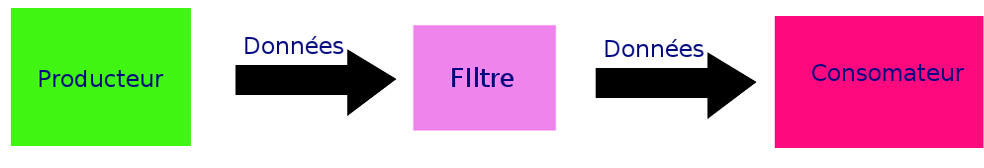
\includegraphics[width=0.95\textwidth]{images/producerConsumer}

  \end{center}

  \caption{Schéma du concept de producteur, filtre, consommateur}

  \label{Yes}

\end{figure}

Le producteur a pour rôle de produire des données (lire un fichier
audio, vidéo\ldots) et de les faire passer au consommateur qui lui est
connecté. Le consommateur a pour but de faire passer ces données (output
datas) à la carte son, device vidéo, un autre fichier, où retransmettre
à travers d'un moyen de télécommunication (broadcasting).%CETTE DERNIERE PHRASE N4EST PAS CLAIRE  
Le filtre
qui n'est pas obligatoire %pour lire des donnés multimedias, permet
de modifier les données (par exemple produisant un effet vidéo/audio),
il peut aussi être connecté à plusieurs producteurs, %avec comme exemple
%la production d'une transition entre ceux-ci.

\subparagraph{}

Mais cela ne permet pas la creation d'éditeur de vidéo non linéaire,
mais seulement la lecture et création de fichier. Pour permettre cette
fonctionnalité, la classe multitrack a été mise en place. Celle-ci
permet de gérer plusieurs producteurs et filtres les uns à la suite des
autres. La multitrack contient plusieurs producteurs et les dispose les
%uns à la suite des autres. Ces mêmes producers peuvent aussi provenir
d'une playlist qui est un concept différent, et celles-ci peuvent aussi
être ajoutées directement à un multitrack, et enregistrées sous forme
de fichier de playlist (dans les différents standards existants).

\subparagraph{}

Grâce à la création de ces réseaux de service, il est possible de
créer des timelines complexes, et ainsi créer des logiciels d'édition
vidéo non linéaires. On peut donc schématiser les réseaux de services
de la manière suivante:

\begin{figure} [H]

  \begin{center}

    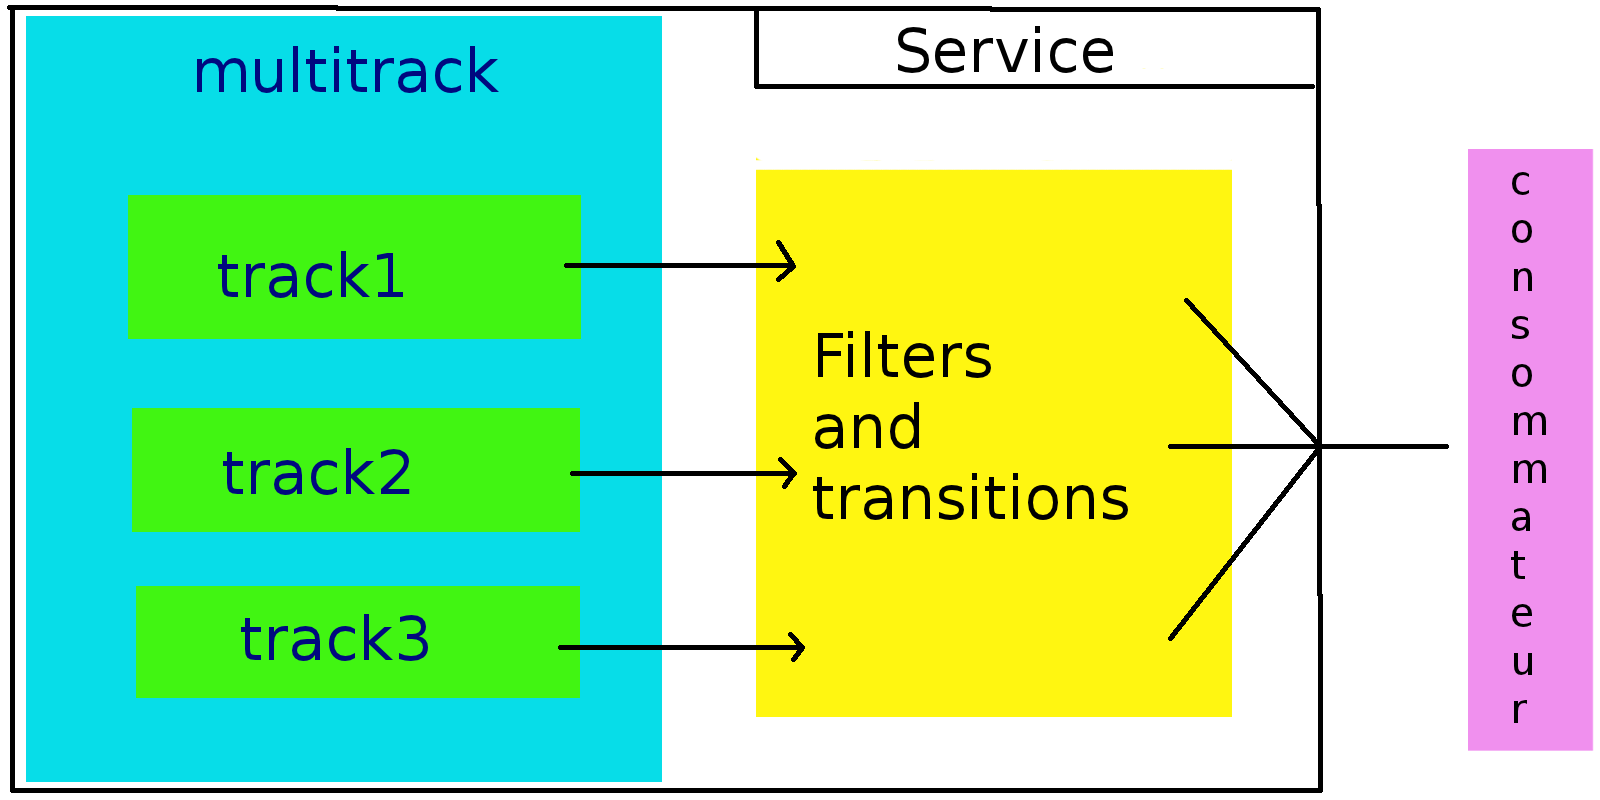
\includegraphics[width=1.0\textwidth]{images/service}

  \end{center}

  \caption{Schéma simplifié d'un service MLT (point de vu interne et
    non utilisateur du framework)}

  \label{Yes}

\end{figure}

\paragraph{Modularité}

\subparagraph{}

Dans MLT, les de producteur, consommateurs où filtres sont des classes
extern implémenté sous form de plugins%INCOMPREHENSIBLE Certains sont implémentés
directement dans MLT tel que :

\begin{itemize}

  \item {Le filtre ``transition'': permet la création de transition}

  \item {Le filtre mono: permet de convertir un flux audio en mono}

  \item {Le filtre resize: Permet de redimensionner une vidéo}

  \item {\ldots}

\end{itemize}

Cela est fait grace à des libraries externes en implémentant des modules
externes afin de faire le lien (wrapper)

\glossary{name={adapter}, description={Il permet de convertir l'interface
d'une classe en une autre interface que le client attend. L' Adaptateur
fait fonctionner ensemble des classes qui n'auraient pas pu fonctionner
sans lui, à cause d'une incompatibilité d'interfaces. Source:
Wikipedia}} entre ces librairies et l'API\index{API} précédemment
présenté. Les principales libraries actuellement utilisables à travers
de ce framework sont:

\begin{itemize}

  \item {libav, libdv et libvorbis pour ce qui %concerne des codecs et
  muxers/demuxers}

  \item {frei0r pour les effets vidéos}

  \item {ladspa pour les effets audios}

  \item {\ldots}

\end{itemize}

\subparagraph{}

Ces différents services disponibles permettent de lire un nombre
considérable de formats multimedia, en particulier grâce à libav,
et d'effectuer de très nombreuses operations principalement grâce aux
plugins frei0r pour la vidéo et ladspa pour l'audio.

\paragraph{Gestion des services}

\subparagraph{Le ``repository``}

%Pour connaitre les différent services
présents sur le système, %l'utilisateur va à sa disposition une classe Repository. Celle-ci
offre une API\index{API} simple listant les différents services par type
(consommateur, producteur ou filtre).  %Pour illustrer, le simple code
suivant permet de récupérer la liste de tous les effets présents
sur le système:

\subparagraph{}

\begin{lstlisting}
  mlt_repository repo = mlt_repository_init (NULL) /* We just use the
  standard module path */ mlt_properties filters = mlt_repository_filters
  (repo); /*
\end{lstlisting}

\subparagraph{Les ``factory''}
%Dans le but de simplifier la création de services de différents
types, MLT utilise le design pattern de la factory. %On peut ainsi
créer n'importe quel type de service de manière simple en utilisant les
différentes factories existantes. Bien que tous les objets d'un réseau
de service soient des descendants de la classe Service, les développeurs
ont décidé de créer 4 méthodes différentes de la classe factory:

\begin{itemize}

  \item {mlt\_factory\_producer: permet d'instancier des producteurs}

  \item {mlt\_factory\_filter: permet d'instancier des filtres}

  \item {mlt\_factory\_transition: permet d'instancier des transitions}

  \item {mlt\_factory\_consumer: permet d'instancier des consommateurs}

\end{itemize}

\subparagraph{}

Par exemple, %pour créer un effet ``invert'' depuis MLT il suffit
de faire:

\subparagraph{}

\begin{lstlisting}
  filter = mlt_factory_filter ( "invert", "my-invert-effect");
\end{lstlisting}

Il sera ensuite possible d'ajouter ce service au réseau de service.

\subparagraph{Les données dans un réseau de services}

\subparagraph{La classe Frame}

\subparagraph{}

Les données qui transitent dans un réseau de service sont contenues dans
des objets de type frame. Celles-ci contiennent à la fois les données
audio et les données vidéos. Les producteurs peuvent setter ces données
grâce aux méthodes mlt\_frame\_set\_audio et mlt\_frame\_set\_video.

\subparagraph{Relations entre les différents services en terme de flux
de données}

Afin commencer le flux de données dans un réseau de service, le
consommateur est celui qui tire les données depuis le service sur
lequel il est connecté.%JE NE COMPRENDS PAS LA PHRASE PRECEDENTE  Les autre services réagissent en fonction,
et formeNT une chaine jusqu'au producteur qui produit les données, et
les fait suivre au service suivant? et ainsi de suite. Ce processus peut
être schématisé de la manière suivante:

\begin{center}

  \begin{tabular}{ | c | c | c | c |}

    \hline

      Phase & producteur              & Filtre                      &
      Consommateur    \\ \hline \hline

      1     &                         &                             &
      Request frame   \\ \hline 2     &                         &
      Réception de la demande     &                 \\
            &                         & Demande la frame à son tour&
            \\ \hline
      3     & Réception de la demande &                             & \\
            & Génération de la frame à la position &                &
            \\ & Mise à jour de la position          &                &
            \\ & Mise à disposition de la frame       &                &
            \\ \hline
      4     &                         & Réception de la frame       & \\
            &                         & Update de la frame          &
            \\ & & Mise à disposition          & \\ \hline
      5     &                         &                             &
      Réception et    \\
            &                         &                             &
            process de      \\ &                         & & la
            frame        \\

    \hline

  \end{tabular}

\end{center}

\subparagraph{}

Cette manière de fonctionner implique que seul le consommateur est
le moteur du réseau. Il est celui qui doit faire partie d'un thread
séparé et les appels à la fonction get\_frame doivent être faits dans
une boucle principale.  Ces appels s'arrêteront au moment où le flux a
été terminé (EOS).


\paragraph{Accélération materiel(%le??)}

\subparagraph{}

Au niveau de l'accélération materiel, MLT supporte le decoding
avec accéleration matériel pour les cartes graphiques Nvidia
\glossary{name={Nvidia}, description={Nvidia Corporation est l'un des plus
grands fournisseurs de processeurs graphiques, de cartes graphiques et de
chipsets pour PC et consoles de jeux}} (via VDPAU), et pour l'affichage
mais pas le compositing vidéo accéléré.

\glossary{name={VDPAU}, description={VDPAU (Video Decode and Presentation
API for Unix) est une bibliothèque open source (libvdpau) et une
interface de programmation conçus par NVIDIA initialement pour ses
cartes graphiques GeForce 8 et ses derniers processeurs graphiques. Cette
interface permet à des programmes de vidéo de décharger de la mémoire
des parties du processus de décodage de vidéo et de son traitement
aval vers le processeur graphique.}}

\paragraph{Fonctionnalités haut niveau (High level features)}

\subparagraph{}

La petite API qu'offre ce framework comporte des méthodes et des fonctions
haut niveau et permet de répondre à des besoins spécifiques de
l'édition vidéo de manière simple pour l'utilisateur.

\subparagraph{Génération de waveform/thumbnail depuis une frame}

\subparagraph{}

Le framework offre par example une fonction permettant la génération
(sous forme d'image) des waveform de la partie audio d'une frame, et de
thumbnail depuis la partie audio.  Dans la partie précédente, nous
avons constaté que la visualisation avancée de chaque frame était une
fonctionnalité très utile en particulier dans le cadre de la création
de films.

\subparagraph{Serialization et deserialization de projets}

\subparagraph{}

Il intègre un système de serialisation, deserialisation, ce qui permet
de sauvegarder facilement les projets, avec les différents tracks,
effets, transition\ldots dans le cadre d'application de montage vidéo.

\subparagraph{}

Le framework MLT offre des bindings haut niveau pour les languages:
C++, C\#, Java, Lua, Perl, PHP, Ruby, TCL et Python. Cela permet à
%un plus grand nombre de développeurs d'envisager l'utilisation de MLT dans
leurs applications. C'est %grâce au binding C++ que Kdenlive a pu être
développé au dessus du framework\index{framework} MLT

\paragraph{Fonctionnalités}

\subparagraph{ }

Cette analyse technique du projet MLT nous permet de constater que
son fonctionnement est simple, et son API petite, et facile à prendre
en main.  Il permet de répondre à différents besoins de base  des
professionnels en terme de fonctionnalités:

\begin{itemize}

  \item {Ajout de titres et génériques: A travers du module développé
  par la
    communauté Kdenlive: QImage.}

  \item {Gestion des keyframes: possible dans les modules implémentant
    cette fonctionnalité, pas de solution générique au niveau du
    core de MLT}

  \item {Visualisation image par images et waveform: Directement
  accessible à
    travers du core de MLT.}

  \item {Visualisation image par image et waveform: Directement
  accessible à
    travers du core de MLT.}

\end{itemize}

\subparagraph{}

La principale %lacune en terme de fonctionnalité est l'impossibilité de
faire du time remapping, mais il est tout de même possible de gérer le
contrôle de la vitesse de lecture des clips, ce qui est un point essentiel.

\subsubsection {Logiciel de montage vidéo basé sur MLT: Kdenlive}

\subparagraph{}

Kdenlive est l'éditeur vidéo créé par la communauté en charge
du bureau libre KDE. Ce logiciel est donc écrit en C++ utilisant le
framework graphique QT \glossary{name={QT}, description={framework
orienté objet et développé en C++ par Qt Development Frameworks,
filiale de Nokia. Il offre des composants d'interface graphique (widgets),
d'accès aux données, de connexions réseaux, de gestion des fils
d'exécution, d'analyse XML, etc. Qt est par certains aspects un framework
lorsqu'on l'utilise pour concevoir des interfaces graphiques ou que l'on
architecture son application en utilisant les mécanismes des signaux
et slots par exemple.}} ainsi que les kdelibs qui forment le framework
permettant la création d'application intégré au bureau du même nom.
L'analyse technique de ce logiciel n'a pas vraiment d'intérêt %car
%on est en présence d'une interface graphique tirant partit du framework MLT.

\paragraph {Interface Graphique}

\subparagraph{}

Il conviendra de présenter succinctement cette interface,
pour ce voici un screenshot:%PAS TRES COMPREHENSIBLE

\subparagraph{}

\begin{figure}[H]

  \begin{center}

    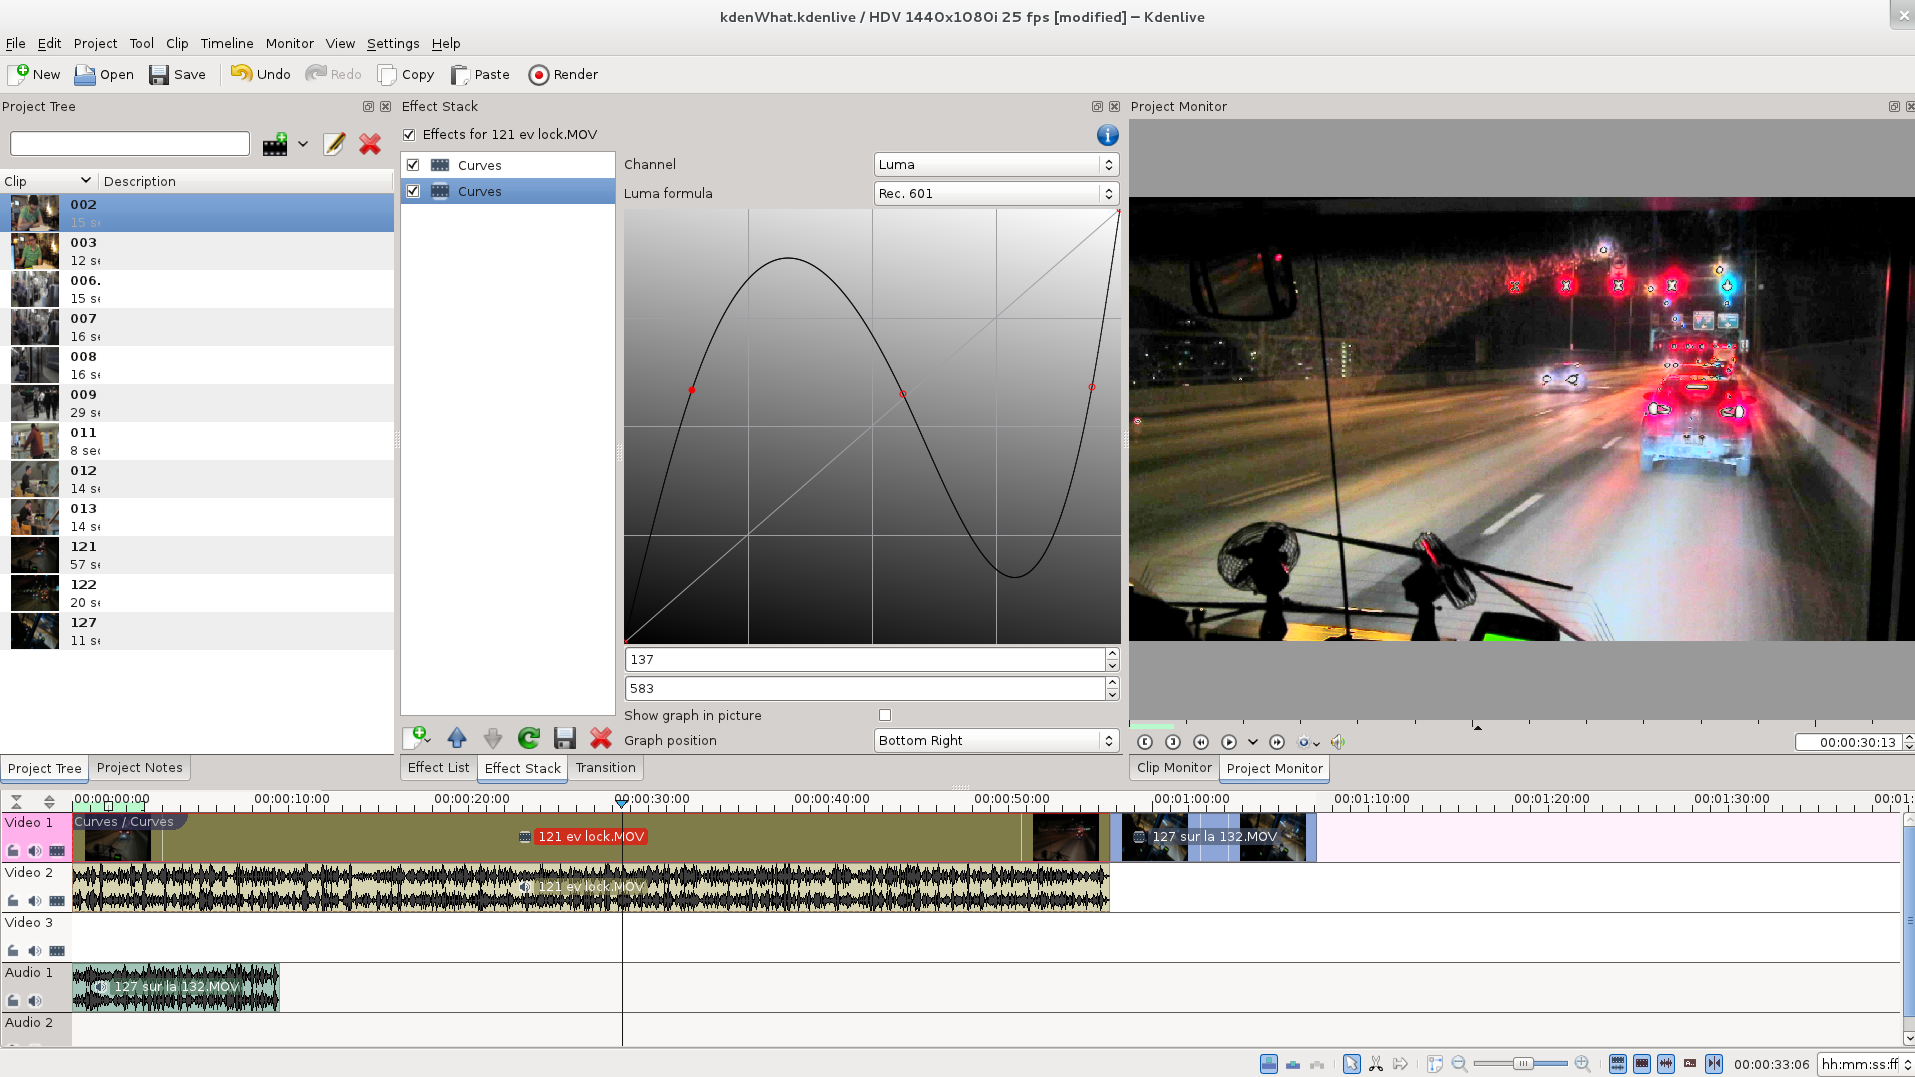
\includegraphics[width=0.90\textwidth]{images/kdenlive}

  \end{center}

  \caption{Screenshot de Kdenlive}

  \label{Yes}

\end{figure}

L'interface graphique de Kdenlive est composé d'une seule fenêtre 
%présentant quatre éléments majeurs:

\begin{itemize}

  \item {La timeline en bas}

  \item {La gestion des footages, en haut à gauche}

  \item {La gestion des effets et transitions, au centre en haut. La
  configuration de ceux-ci se fait dans cette même partie.}

  \item {Le previewer, en haut à droite}

\end{itemize}

\subsection {PiTiVi}

Comme précédemment énoncé, PiTiVi utilise le framework multimedia
GStreamer. Dans cette partie, nous nous concentrerons sur l'analyse
de ce framework.

\subsubsection {Framework multimedia: GStreamer}

\paragraph {Panorama de la technologie} %Overview?

\subparagraph{}

GStreamer un framework multimedia basé sur le concept de pipeline
écrit en C.  L' API de ce framework est plus complet que celle de
MLT puisque les use-cases auxquels celui- ci cherche à répondre sont
plus nombreux. En effet, la communauté GStreamer a pour objectif de
créer un framework open source permettant de répondre au plus grand
nombre possible de cas d'utilisations ayant un lien avec le multimedia
(depuis les téléphones mobiles jusqu'aux renders farms en passant par les
logiciels de montage video).  Ce framework, bien qu'écrit en C,
utilise le paradigme objet, à travers de la librairie Glib. Cette
librairie implémente de nombreuses API et en particulier la notion
d'objet en C à travers le? module GObject. La Glib permet aussi la
gestion des threads, des signaux\ldots De très nombreux projets
de logiciels libres l'utilisent, en particulier le projet d'interface
graphique Gnome. GStreamer offre une API stable aussi bien pour les
développeurs de plugins que pour les développeurs d'applications. Il
est hautement multi threaded\glossary{name={thread}, description={Il
s'agit de la plus petit unité de processus qui peut être exécutée par un
système d'exploitation. Ils permettent à un même ``programme'', processus
d'exécuter du code de manière concurrente.}}, et est thread safe,
c'est a dire que la mémoire partagée par les differents threads ne
peut pas être corrompue dans le cas ou plusieurs threads voudraient la modifier
en même temps(en utilisant le système d'exclusion mutuel).

Le schéma suivant permet de représenter graphiquement l'architecture
globale du framework:

\begin{figure} [H]

  \begin{center}

    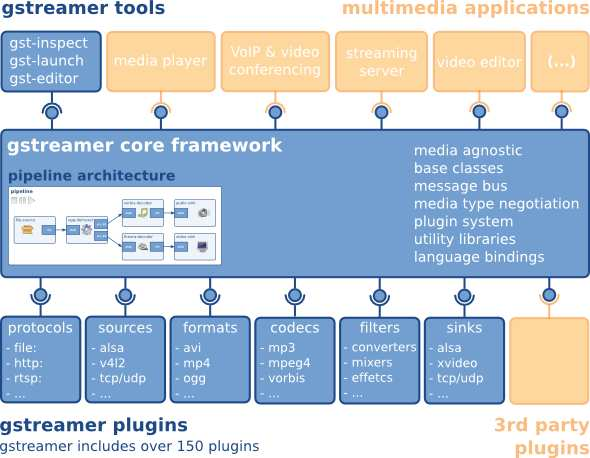
\includegraphics[width=0.95\textwidth]{images/gstoverview}

  \end{center}

  \caption{Architecture du framework GStreamer}

  \label{Yes}

\end{figure}

\subparagraph{}

GStreamer est distribué sous licence LGPL Version

\paragraph{Concepts de base}

\subparagraph{Le concept de pipeline}

\subparagraph{}

La grande majorité des classes dans GStreamer dérive de la classe
GstElement qui est l'élément de base dans un pipeline, lui même
GstElement. Un schéma permet d'expliquer cette notion de pipeline assez
facilement:

\begin{figure} [H]

  \begin{center}

    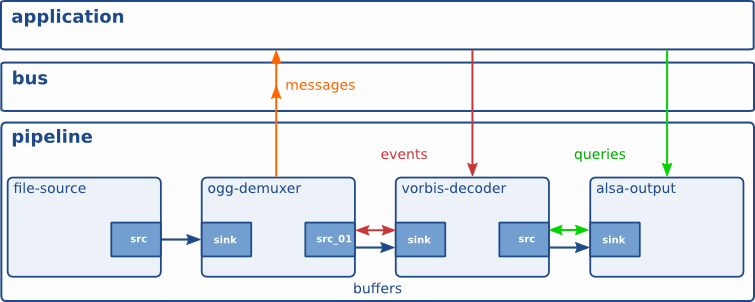
\includegraphics[width=0.95\textwidth]{images/gstpipeline}

  \end{center}

  \caption{Un pipeline GStreamer permettant la lecture d'un fichier
  audio ogg
    ayant pour codec vorbis (ce schéma prend en compte d'autres notions
    importantes du framework).}

  \label{Yes}

\end{figure}

\subparagraph{}

On constate que l'architecture est assez similaire à celle MLT, avec
pour grande difference le fait que les éléments composants le ``réseau
de service'' sont tous dans un même élément: le pipeline. Cet élément
GStreamer éxécute un thread séparé à partir du moment où l'on cherche a
jouer son contenu. Dès lors, les données transitent entre les différents
élément gstreamer, a commencé par l'élément source. Dans l'exemple
donne par ce schéma, il s'agit d'un file-source, et terminant par le
sink, dans notre exemple alsa-output. Les éléments entre les deux se
chargent du demuxing (ogg-demux), et du decoding (vorbis-decoder).

\subparagraph{}

Une autre différence réside dans le fait que l'utilisateur de
GStreamer a un contrôle plus important que dans le cas de MLT sur
les composants de la chaines d'éléments permettant la reproduction de
contenu multimedia.  Dans GStreamer chaque tâche est effectuée par un
élément, c'est à dire qu'un service MLT sera décomposé en plusieurs
élément GStreamer. Dans le cadre d'un producteur en particulier, chez
GStreamer, cela est effectué à travers un élément pour chaque étape
du coding/decoding/muxing/demuxing, et dans certain cas, du parsing du
bitstream. Cette décomposition en petits éléments effectuants une tâche
a le gros avantage de permettre la réutilisabilité de chacun d'eux et
ce, dans les différents  contextes d'applications multimédia.

\subparagraph{Communication entre les éléments}

\subparagraph{}

La communication entre ces différents éléments se fait au travers des
GstPad. Il convient de représenter un élément (dans ce cas un démuxer,
qui permet de recevoir un flux en entrée de le décomposer afin d'avoir
deux sorties, l'une contenant les données audios, et l'autre avec les
données vidéos), de la manière suivante:

\begin{figure} [H]

  \begin{center}

    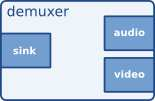
\includegraphics[width=0.30\textwidth]{images/gstdemuxer}

  \end{center}

  \caption{Représentation graphique d'un GstElement permettant le
  demuxing.}

  \label{Yes}

\end{figure}

Sur ce schéma, on constate la présence d'un sink pad, nommé ``sink'',
et deux sources pad, nommées ``audio'' et ``video''. Ces objets permettent
la connection entre les différents éléments. Ils peuvent être comparés
aux ``prise'' et ``port'' dans le monde réel.  Afin de brancher une prise
dans un port, il convient de s'assurer que ceux-ci soient compatibles,
%CE QUI SUIT EST INCOMPREHENSIBLE
c'est ce but qu'on les caps, assurer la compatibilité de la communication
entre différents éléments.

\paragraph {Modularité}

\subparagraph{}

GStreamer est extrêmement modulaire, et l'on peuT l'étendre facilement
en créant de nouveaux éléments. Il suffit d'ajouter ces élément (sous
forme de plugins) sur le système pour que l'utilisateur puisse tirer
partie des nouvelles fonctionnalités. La communauté GStreamer offre des
collections de plugins contenant un très grand nombre d'élément. Ces
set de plugins sont classés selon des critères précis:

\begin{itemize}

  \item {base: Plugins de grande qualité et très bien maintenus. Il
  offre aussi
    des classes de base afin de faciliter la creation d'éléments.}

  \item {good: Plugins de qualité, ayant une licence LGPL}.

  \item {Ugly: Plugins de qualité, ayant des problèmes au niveau de
  la licence.}

  \item {bad: Plugins de moins grande qualité, ayant des problèmes
  au niveau
    de la licence. Il s'agit d'éléments dont le code a été
    moins testé et risque ainsi de %présenter davantage de bugs.}

\end{itemize}

\subparagraph{}

De nombreuses librairies sont wrapper dans ces différentes collections de plugins, par exemple, dans ``bad'', les librairies d'effets ladspa
et frei0r y sont incluses et %dès qu'elles sont
installées sur le système, %elles permettent à n'importe quelle application basée GStreamer
de bénéficier de leurs fonctionnalités.  Ces plugins sont distribués
sous forme de librairies partagées, et peuvent donc être chargées à la
volée, durant l'exécution du framework.

\subparagraph{}

En terme de lecture de contenu multimedia, les développeurs GStreamer
conseillent l'utilisation de la collection de plugins ``gst-ffmpeg''
qui permet de bénéficier de toutes les codec, muxer et demuxer de cette
librairie. D'autres librairies tel que libogg, libdv, x264\ldots sont
wrapper dans les différentes collections de plugins précédemment
présentées.

\paragraph{Gestion des éléments}

\subparagraph{}

La gestion des éléments est très comparable à ce qui est fait
dans le framework MLT, c'est à dire, que l'on a une classe GstRegistry
(comparable à la classe repository de MLT), et des GstFactory qui permettent
la fabrication facile d'éléments.

\paragraph{Et l'édition vidéo?}

\subparagraph{}

En effet, tout cela ne nous permet pas de faire  de l'édition vidéo%
%requiert la création de pipeline dynamique, c'est
%à dire qui permet de faire évoluer les éléments présents dans le
pipeline au fil du temps.  %C'est pour cette raison que les éléments du plugins Gnonlin
ont été développés. Il s'agit de 4 éléments principaux %dont voici la définition

\begin{itemize}

  \item {GnlComposition: élément le plus important qui permet de
  faire évoluer
    le pipeline de manière dynamique}

  \item{Gnl[uri/file]Source: élément source qui a les propriétés
    nécessaires pour savoir à quel moment il doit être présent ou
    non dans le pipeline}

  \item{GnlOperation: élément qui permet l'application d'effet, transition
    etc\ldots il a aussi les propriété %de savoir à quel moment il
    doit être présent ou non dans le pipeline}
%IL MANQUE UNE QUATRIEME DEFINITION....

\end{itemize}

\subparagraph{}

Mais ces éléments ne permettent pas de facilement créer des applications de
montage audio/ou vidéo. Le core actuel de PiTiVi utilise directement ces
éléments afin de gérer les notions propres à l'édition vidéo, mais les développeurs
se sont rendu compte que cela était trop complexe à utiliser, et par conséquent
PiTiVi n'est pas une simple interface au dessus de GStreamer, mais introduit 
plusieurs concepts supplémentaires au dessus de ces éléments.

\newpage \section{Analyse des communautés}

\newpage \section{Lacunes}

\newpage \section{Solutions possibles}
